


%% Goal is 

% \section{Introduction}
% \label{sec:GUI:introduction}
% \SweaveInput{Introduction}


\XXX{Space}
\XXX{HCI}
\XXX{http://www.useit.com/alertbox}
\XXX{Apple HIG}
\XXX{comment on radio vs. check http://www.useit.com/alertbox/20040927.html}
\section{A simple GUI in R}
\label{sec:GUI:tic-tac-toe}
%% Tic Tac Toe examples

We begin with an example showing how one can use \R's standard
graphics device as a canvas for a ``game'' of
tic-tac-toe against the computer (Figure~\ref{fig:basics-tic-tac-toe}). Although this example
has nothing to do with statistics, it illustrates, in a familiar way,
some of the issues involved in developing GUIs in \R. 


%% ML: the note about the MVC pattern can probably come after the
%% concrete model, view and controller have been presented. We can
%% look back and point out that the design of the example can be
%% generalized to MVC and that we will encounter such designs
%% throughout the book, even if it is not always explicit. It's OK to
%% generalize a little after each step, but I think we want to lead
%% with the concrete.

Generally, GUIs provide the means for viewing and controlling some
underlying data structure.  In this example, the data simply consists
of information holding the state of the game, defined here in a global
variable \code{board}.

%% Model
\begin{Schunk}
\begin{Sinput}
 board <- matrix(rep(0,9), nrow=3)      
\end{Sinput}
\end{Schunk}

%% View
A GUI contains one or more views, each of which displays the data in a
particular manner.  In our case, the view is the game board that we
display through an \R\/ graphics device. The \function{layoutBoard}
function creates a canvas for this view:
\begin{Schunk}
\begin{Sinput}
 layoutBoard <- function() {
   plot.new()
   plot.window(xlim=c(1,4), ylim=c(1,4))
   abline(v=2:3);  abline(h=2:3)
   mtext("Tic Tac Toe. Click a square:")
 }
\end{Sinput}
\end{Schunk}
%
This example uses a single view; more complex GUIs
will contain multiple coordinated, interactive views. The layout of
the GUI should help the user navigate the interface and is an
important factor in usability. Here we benefit from the universal
familiarity with the board game.


%% Controller
The user typically sends input to a GUI through a mouse or keyboard. 
The underlying toolkit allows the programmer to assign
functions to be called when some specific event occurs, such as user interaction. Typically, the
toolkit \igui{signals}\textit{signals} that some action has occurred, and then
invokes \igui{event handlers}\textit{callbacks} or \textit{event handlers} that have been
assigned by the programmer. Each toolkit has a different implementation. 
For our game, we will use the \code{locator} function built
into the base \R\/ graphics system:
\begin{Schunk}
\begin{Sinput}
 doPlay <- function() {
   iloc <- locator(n=1, type="n")
   clickHandler(iloc)
 }
\end{Sinput}
\end{Schunk}
%
The \code{locator} function responds to mouse clicks. One specifies
how many mouse clicks to gather and the \textit{control} of the
program is suspended until the user clicks the sufficient number of
times (or somehow interrupts the loop). Such a GUI that enters a mode
in which the flow of a program is blocked and waiting on user input is
known as a \igui{modal dialogs}\textit{modal} GUI. This design is
common for simple dialogs that require immediate user attention,
although in general a GUI will listen asynchronously for user input.

\begin{figure}
  \centering
  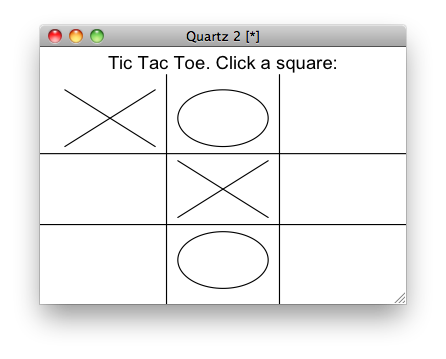
\includegraphics[width=.6\textwidth]{fig-basics-tic-tac-toe}
  \caption{Using a graphics device for a game of tic-tac-toe}
  \label{fig:basics-tic-tac-toe}
\end{figure}



In the above function \function{doPlay}, \function{clickHandler} is
an \defn{event handler}. Its job is to process the output of the
\function{locator} function, checking first if the user terminated
\function{locator} using the keyboard. If not it proceeds to draw the
move, and then, if necessary, the computer's move. Afterwards, play is
repeated until there is a winner or a ``cat's'' game.


\begin{Schunk}
\begin{Sinput}
 clickHandler <- function(iloc) {
   if(is.null(iloc)) 
     stop("Game terminated early")
   move <- floor(unlist(iloc))
   drawMove(move,"x")
   board[3*(move[2]-1) + move[1]] <<- 1
   if(!isFinished()) 
     doComputerMove()
   if(!isFinished()) 
     doPlay()
 }
\end{Sinput}
\end{Schunk}

The use of \verb+<<-+ in the handler illustrates a typical issue in
GUI design in \R.  User input changes the state of the application
through callback functions. These callbacks need to modify variables
\iprogram{variable scope}in some shared scope, which may be
application-wide or specific to a component. The lexical scoping rules
of \R, i.e., nesting of closures, has proven to be a useful strategy
for managing GUI state. In the above case, we simply modify the global
environment, which encloses \function{clickHandler}. When this is
inconvenient, direct manipulation of environment objects is sometimes
a feasible option. If the scale of the GUI demands more formal
mechanisms, we recommend the reference class framework from the
\pkg{methods} package.

%% validation of user input
\iprogram{validation}Validation of user input is an important task for a GUI. In the above,
the \function{clickHandler} function checks to see if the user
terminated the game early and issues a message.

%% Implement logic
At this point, we have a data model, a view of the model and the
logic that connects the two, but we still need to implement some of the
functions to tie it together.


This function draws either an ``x'' or an ``o''. It does so using the
\function{lines} function. The \code{z} argument contains the
coordinates of the square to draw.
\begin{Schunk}
\begin{Sinput}
 drawMove <- function(z,type="x") {
   i <- max(1,min(3,z[1])); j <- max(1,min(3,z[2]))
   if(type == "x") {
     lines(i + c(.1,.9),j + c(.1,.9))
     lines(i + c(.1,.9),j + c(.9,.1))
   } else {
     theta <- seq(0,2*pi,length=100)
     lines(i + 1/2 + .4*cos(theta), j + 1/2 + .4*sin(theta))
   }
 }
\end{Sinput}
\end{Schunk}

%% Resizing
One could use \code{text} to place a text ``x'' or ``o'', but this may
not scale well if the GUI is resized. Most GUI layouts allow for
\ilayout{resizing}dynamic resizing. This is necessary to handle the variety of data a
GUI will display. Even the labels, which one generally considers
static, will display different text depending on the language (as long
as translations are available).

%% JV: thanks
This function is used to test if a game is finished:
\begin{Schunk}
\begin{Sinput}
 isFinished <- function() {
   (any(abs(rowSums(board)) == 3) || 
    any(abs(colSums(board)) == 3) || 
    abs(sum(diag(board))) == 3 || 
    abs(sum(diag(apply(board, 2, rev)))) == 3)
 }
\end{Sinput}
\end{Schunk}
%
The matrix \code{m} allows us to easily check all the possible ways
to get three in a row.

This function picks a move for the computer:
\begin{Schunk}
\begin{Sinput}
 doComputerMove <- function() {
   newMove <- sample(which(board == 0),1) # random !
   board[newMove] <<- -1    
   z <- c((newMove-1) %% 3, (newMove-1) %/% 3) + 1
   drawMove(z,"o")
 }
\end{Sinput}
\end{Schunk}
%
The move is converted into coordinates using \code{\%\%} to get the
remainder and \code{\%/\%} to get the quotient when dividing an
integer by an integer. This function just chooses at random from the
left over positions; we leave implementing a better strategy to the
interested reader.

%% main equivalent
Finally, we implement the main entry point for our GUI:
\begin{Schunk}
\begin{Sinput}
 playGame <- function() {
   board <<- matrix(rep(0,9), nrow=3)  
   layoutBoard()
   doPlay()
   mtext("All done\n",1)
 }
\end{Sinput}
\end{Schunk}
%
When the game is launched, we first lay out the board and then call
\function{doPlay}. When \function{doPlay} returns, a message is written
on the screen.

This example adheres to the model-view-controller design pattern that
is implemented by virtually every complex GUI. We will encounter this
pattern throughout this book, although it is not always explicit.

%% endless tweak
For many GUIs there is a necessary trade-off between usability and
complexity. As with any software, there is always the temptation to
continually add features without regard for the long term cost. In
this case, there are many obvious improvements: implementing a better
artificial intelligence, drawing a line connecting three in a row when
there is a win, indicating who won, etc. Adding a feature increases
the functionality, at the cost of increased complexity and burden on
the user.

\section{GUI Design Principles}
\label{sec:GUI:design}
% Section to introduce GUI design and principles through a comparison of
% three dialogs and general discussion


%% mac defs:

% Document windows contain file-based user data. They present a view
% into the content that people create and store. If the document is
% larger than the window, the window shows a portion of the document’s
% contents and provides users with the ability to scroll to other areas.

% Application windows are the main windows of applications that are not
% document-based. These windows can use the standard Aqua window look
% and features or (less frequently) the brushed metal look.

% Utility windows float above other windows and provide tools or
% controls that users can work with while documents are open. Utility
% windows (also called palettes) are discussed in more detail
% in “Utility Windows.” (page 202)

% Dialogs and alerts require a response from the user. These are
% discussed in “Dialogs.” (page 207)


The most prevalent pattern of user interface design is denoted WIMP,
which stands for Window, Icon, Menu and Pointer. The
WIMP approach was developed at Xerox PARC in the 1970's and later
popularized by the Apple Macintosh in 1984. This is particularly
evident in the separation of the window from the menubar on the Mac
desktop. Other graphical operating systems, such as Microsoft Windows,
later adapted the WIMP paradigm, and libraries of reusable GUI
components emerged to support development of applications in such
environments. Thus, GUI development in R adheres to the WIMP approach.

The primary WIMP component from our perspective is the window. A
typical interface design consists of a \igui{top-level window}top-level window referred to as
the \dfnref{document window} that shows the current state of a
``document,'' whatever that is taken to be. In \R\/ it could be a data
frame, a command line, a function editor, a graphic or an arbitrarily
complex form containing an assortment of such elements. 

%% JV: control or "action" here?
%% ML: tried to make this clearer

Abstractly, WIMP is a command language, where the user executes
commands, often called actions, on a document by interacting with
graphical controls. Every control in a window belongs to some abstract
menu. Two common ways of organizing controls into menus are the
menubar and toolbar.

The parameters of an action call, if any, are controlled in
sub-windows. These sub-windows are termed \dfnref{application windows}
by Apple\footcite{APPLE:HIG}, but we prefer the term \igui{dialogs}\dfnref{dialogs},
or \dfnref{dialog boxes}. These terms may also refer to smaller
sub-windows that are used for alerts or confirmation. The program
often needs to wait for user input before continuing with an action,
in which case the window is modal. We refer to these as \dfnref{modal
  dialog boxes}.

Each window or dialog typically consists of numerous controls laid out
in some manner to facilitate the user interaction. Each window and
control is a type of \textit{widget}, the basic element of a
GUI. Every GUI is constituted by its widgets. Not all widgets are
directly visible by the user; for example, many GUI frameworks employ
invisible widgets to lay out the other widgets in a window.

There is a wide variety of available widget types, and widgets may be
combined in an infinite number of ways. Thus, there are often numerous
means to achieve the same goals. For example,
Figures~\ref{fig:GUI:print-dialogs} and \ref{fig:GUI:print-dialogs-R}
show three dialogs, representing typical dialogs from the three main
operating systems, that perform the same task -- collect arguments
from the user to customize the printing of a document. Although all
were designed to do the same thing, there are many differences in
implementation.

%% ML: Print dialogs might be problematic, especially with Firefox, which
%% (through GTK+) will use the platform native print dialog. On Linux,
%% there is no native dialog, so GTK+ implements one. This might not
%% be true of Firefox 2.0 specifically, but that is getting old
%% now. What about taking the print dialog from the R Windows GUI?

%% Principles of GUI layout
%% http://www.sylvantech.com/~talin/projects/ui_design.html has a nice list

\begin{figure}
  \centering
  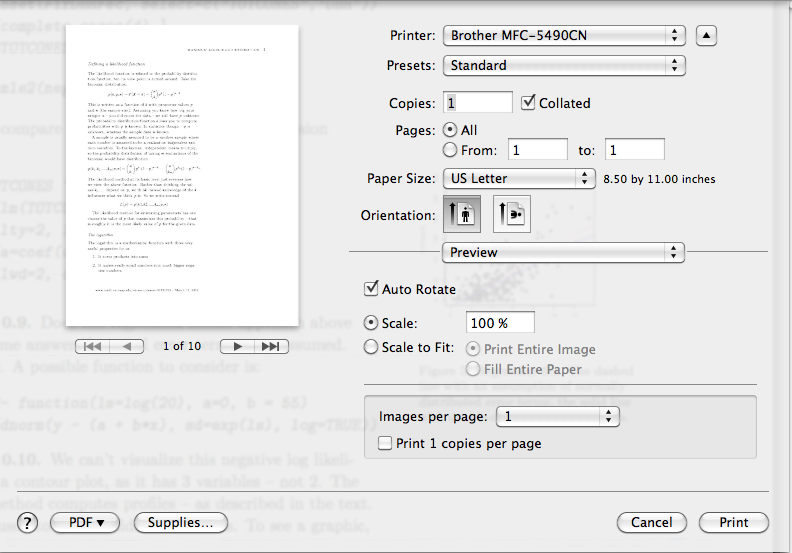
\includegraphics[width=.75\textwidth]{fig-mac-print}
   \\
   
  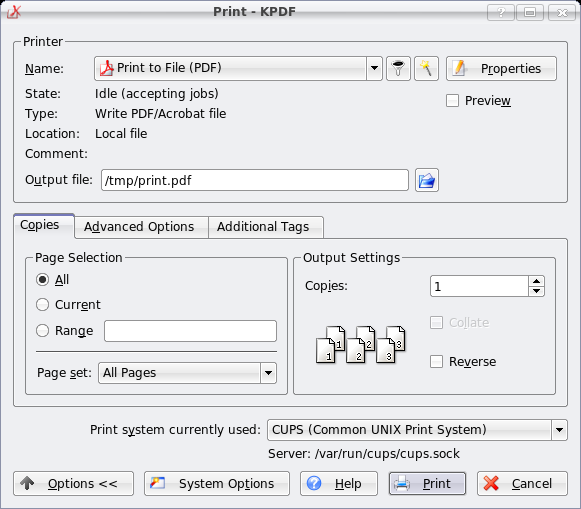
\includegraphics[width=.75\textwidth]{kde-print}
  \caption{Two print dialogs. One from Mac OS X 10.6 and one from KDE 3.5.}
  \label{fig:GUI:print-dialogs}
\end{figure}


\begin{figure}
  \centering
  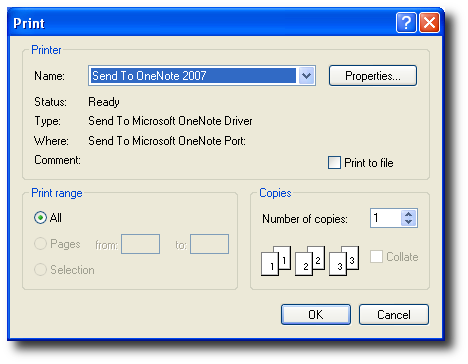
\includegraphics[width=.80\textwidth]{r-print-dialog}
  \caption{\R's print dialog under Windows XP using XP's native dialog.}
  \label{fig:GUI:print-dialogs-R}
\end{figure}

%% Choice of widget -- familiar metaphors, use of icons, 
In some cases, typical usage suggests one control over another. The
choice of printer for each is specified through a combo box. However,
for other choices a variety of widgets are employed. For example, the
control to indicate the number of copies for the Mac is a simple text
entry window, whereas for the KDE and Windows dialog it
is a spin button. The latter provides a bit more functionality, for a
bit more complexity. The KDE and Mac dialogs have icons to
compactly represent actions, whereas the the Windows example has none. The
landscape icon for the Mac is very clear and provides this feature
without having to use a sub dialog.


%% Choice of layout -- positioning, focus, use of spacing, center
%% balance, vs. ...
How the interfaces are laid out also varies.  All
panels are read top to bottom, although the Mac interface also has a very
nice preview feature on the left side. The KDE dialog uses frames to
separate out the printer arguments from the arguments that specify how
the print job is to proceed. The Mac uses a vertical arrangement to
guide the user through this. For the Mac, horizontal separators are
used instead of frames to break up the areas, although a frame is used
towards the bottom. Apple uses a center balance for its controls. They
are not left justified as are the KDE and Windows dialogs. Apple has
strict user-interface guidelines and this center balance is a design
decision.

%% feature exposure, Choice of options -- what to show, what to leave out
The layout also determines how many features and choices are visible to the
user at a given time.  For example, the Mac GUI uses ``disclosure
buttons'' to allow access to printer properties and the PDF settings,
whereas KDE uses a notebook container to show only a subset of the
options at once.

%% state visualization: sensitive/not; focus, not, 
The Mac GUI provides a very nice preview of the current document
indicating, to the user clearly what is to be printed and how
much. Adjusting GUIs to the possible state is an important user
interface property.  GUI areas that are not currently sensitive to
user input are grayed out. For example, the ``collate'' feature of the
GUI only makes sense when multiple copies are selected, so the
designers have it grayed out until then. A common element of GUI
design is to only enable controls when their associated action is
possible, given the state of the application.

%% shortcuts -- default button, keyboard accelerators
 
The Mac GUI has the number of pages in focus, whereas Windows places
the printer in focus. Focus allows the user to interact with the GUI
without the mouse. Typically the \kbd{tab} key is used to step through
the controls. GUI's often have shortcuts that allow power users to
initiate actions or shift the focus directly to a specific widget
through the keyboard.  Most dialogs also have a default button, which
will initiate the dialog action when the \kbd{return} key is
pressed. The KDE dialog, for example, indicates that the ``print''
button is the default button through special shading.

%% help
% For such a common dialog, it is unlikely the user will need help. As
% such the Windows dialog does not provide a link. However, the
% KDE and Mac dialogs do. A dialog should provide assistance for
% complex and unfamiliar tasks.

%% safety -- postion of buttons
%% ML: Do we really want to mention something that is not applicable?
%% JV; Agreed
% The Apple human interface guidelines suggest putting buttons that can
% cause the destruction of data separate from other control buttons. As
% this isn't directly applicable here, we see that Apple does separate
% buttons that are common to many dialogs (cancel, print) from the ones
% specific to the dialog. The KDE buttons have nice icons, but their
% similar, but irregular, sizing is a bit unusual.


Each dialog presents the user with a range of buttons to initiate or
cancel the printing. The Windows ones are set on the right and consist
of the standard ``OK'' and ``Cancel'' buttons. The Mac interface uses
a spring to push some buttons to the left, and some to the right to
keep separate their level of importance. The KDE buttons do so as
well, although one cannot tell from the image. The use
of conventional icons on the buttons also help guide the user. 


%% JV should we leave this in? I'm wondering. We do it better in the
%% chapters perhaps
\section{Controls}
\label{sec:GUI:basic-components}
%% ML: This section and the next should probably be reorganized so
%% that they do a better job of referring to examples. Otherwise it
%% feels like we're stating a series of groundless generalities.

This section provides an overview of many common controls, i.e.,
widgets that either accept input, display data or provide visual
guides to help the user navigate the interface. If the reader is
already familiar with the conventional types of widgets and how they
are arranged on the screen, this section and the next should be
considered optional.


\subsection{Choice of control}
\label{sec:choice-widget}
%% real estate, type of data


\begin{table}
\centering
\label{tab:gui-design-widget-type}
\caption{Table of possible selection widgets by data type, size and selection mode (single or multiple)}
\begin{tabular}{@{}lp{0.35\textwidth}p{0.35\textwidth}@{}}
\toprule

Type of data&Single&Multiple\\
\midrule
Boolean&Checkbox, toggle button&-\\Small list&radio button group\newline combo box\newline list box&checkbox group\newline list box\\Moderate list&combo box\newline list box&list box\\Large list&list box, auto complete&list box\\Sequential&slider\newline spin button&\\Tabular&table&table\\Hierarchical&tree&tree
\\ \bottomrule
\end{tabular}
\end{table}
A GUI is comprised of one or more widgets. The appropriate choice
depends on a balance of considerations.  For example, many widgets
offer the user a selection from one or more possible choices.  An
appropriate choice depends on the type and size of the information
being displayed, the constraints on the user input, and on the space
available in the layout. As an example,
Table~\ref{tab:gui-design-widget-type} suggests different types
of widgets used for this purpose depending on the type and size of
data and the number of items to select.
  

Figure~\ref{fig:GUI:spss-11-term-selection} shows several such
controls in a single dialog. A checkbox enables an intercept,
a radio group selects either full factorial or a custom
model, a combo box selects the ``sum of squares'' type, and a
list box allows for multiple selection from the available
variables in the data set. 




%% Metaphors, user base
For many \R\/ object types there are natural choices of widget. For
example, values from a sequence map naturally to a slider or spin
button; a data frame maps naturally to a table widget; or a list with
similar structure can map naturally to a tree widget. However, certain
\R\/ types have less common metaphors. For instance, a formula object
can be fairly complex. Figure~\ref{fig:GUI:spss-11-term-selection}
shows an SPSS dialog to build terms in a model. \R\/ power users may
be much faster specifying the formula through a text entry box, but
beginning \R\/ users coming to grips with the command line and the
concept of a formula may benefit from the assistance of a well
designed GUI. One might desire an interface that balances the needs of
both types of user, or the SPSS interface may be appropriate. Knowing
the potential user base is important.




\begin{figure}
  \centering
  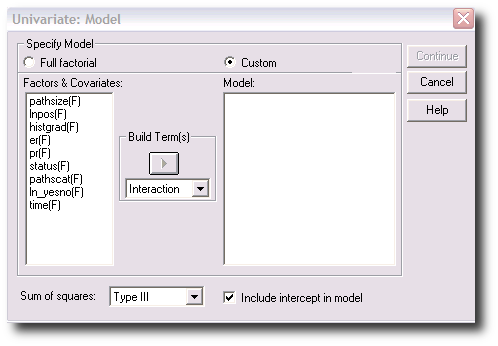
\includegraphics[width=.65\textwidth]{spss-11-formula-editor}
 \caption{A dialog box from SPSS version 11 for specifying terms
    for a linear model. The graphic shows a dialog that allows
    the user to specify individual terms in the model  using
    several types of widgets for selection of values, such as a radio button
    group, a checkbox, combo boxes, and list boxes. }
  \label{fig:GUI:spss-11-term-selection}
\end{figure}


\subsection{Presenting options}
\label{sec:GUI:basic-selection}

The widgets that receive user input need to translate that input into
a command that modifies the state of the application. Commands, like
\R{} functions, often have parameters, or options. For many options,
there is a discrete set of possible choices, and the user needs to
select one of them. Examples include selecting a data frame from a list of data
frames, selecting a variable in a data frame, selecting certain cases
in a data frame, selecting a logical value for a function argument,
selecting a numeric value for a confidence level or selecting a string
to specify an alternative hypothesis. Clearly there can be no
one-size-fits-all widget to handle the selection of a value.

% XXX REDO FIGURE
% \begin{figure}
%   \centering
%   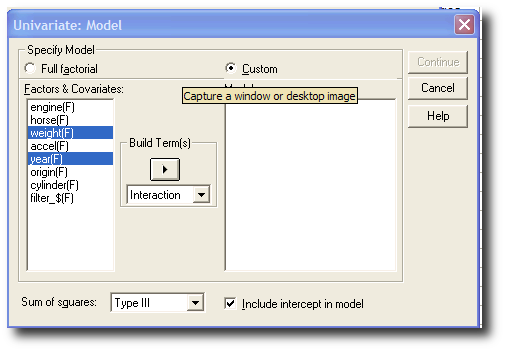
\includegraphics[width=.45\textwidth]{spss-11-model-selection}
%   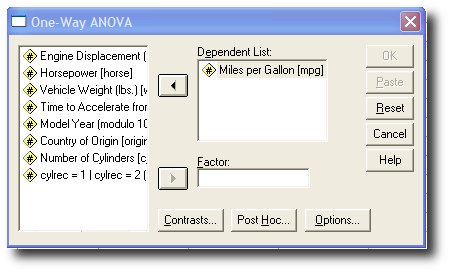
\includegraphics[width=.45\textwidth]{spss-11-one-way-anova}
%   \caption{Two dialog boxes from SPSS version 11 for specifying terms
%     for a linear model. The left graphic shows a dialog that allows
%     the user to specify individual terms in the model. This uses
%     several types of widgets for selection of values, such as a radio
%     group, a checkbox, combo boxes, and list boxes. The right graphic
%     shows a dialog that allows the user to specify response variables
%     and a grouping variable for a one-way ANOVA.}
%   \label{fig:GUI:spss-11-model-selection}
% \end{figure}


\subsubsection{Checkboxes}
\label{sec:GUI:checkboxes}

A \dfn{checkbox} specifies a value for a logical
(boolean) option. Checkboxes have labels to indicate which variable is
being selected. Combining multiple checkboxes into a group allows for
the selection of one or more values at a time.


\subsubsection{Radio buttons}
\label{sec:GUI:radio=button-groups}

A \dfn{radio button group} selects exactly one value from a vector of
possible values. The analogy dates back to old car radios where there
were a handful of buttons to select a preset channel. When a new
button was pushed in, the previously pressed button popped up.  Radio
button groups are useful, provided there are not too many values to
choose from, as all the values are shown. These values can be arranged
in a row, a column or both rows and columns to better fill the
available space. Figure~\ref{fig:GUI:ex-tcltk} uses radio button
groups for choosing the distribution, kernel and sample size for the
density plot.

\subsubsection{Combo boxes}
\label{sec:GUI:combo-boxes}

A \dfn{combo box} is similar to a radio button group, in that it is
used to select one value from several. However, a combo box only
displays the value currently selected, which reduces visual complexity
and saves space, at the cost of an extra click to show the
choices. Toolkits often combine a combo box with a text entry area for
specifying an arbitrary value, possibly one that is not represented in
the set of choices. A combo box is generally desirable over radio
buttons when there are more than four or five choices. However, the
combo box also has its limits. For example, some web forms require
choosing a country from a list of hundreds. In such cases, features
like incremental type ahead search are useful.

\subsubsection{List boxes}

A \dfn{list box} displays a list of possible choices in a column.
While the radio button group and combo box select only a single value,
a list box supports multiple selection. Another difference is that the
number of displayed choices depends dynamically on the available
space. If a list box contains too many items to display them
simultaneously, a scrollbar is typically provided for adjusting the
visible range. Unlike the combo box, the choices are immediately visible
to the user.  Figure~\ref{fig:GUI:ex-tcltk} shows a list
box created by the \R\/ function
\command{chooseCRANmirror}. There are too many mirrors to fit on the
screen, but a combo box would not take advantage of the available
space. The list box is a reasonable compromise.

%% tcltk examples
\begin{figure}
  \centering
  \begin{minipage}[c]{.45\linewidth}
    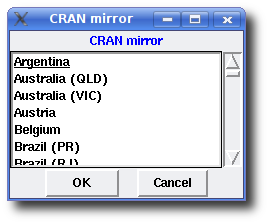
\includegraphics[width=1\textwidth]{ex-listbox}
  \end{minipage}
  \begin{minipage}[c]{.45\linewidth}
    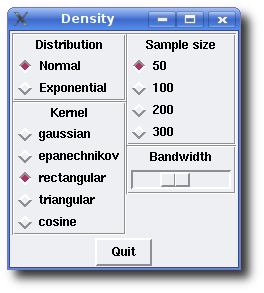
\includegraphics[width=1\textwidth]{tcltk-tkdensity}    
  \end{minipage}
 \caption{
    Two applications of the \pkg{tcltk} package. 
    %% 
    The left graphic is
    produced by \command{chooseCRANmirror} and uses a list box to
    allow selection from a long list of possibilities.
    %% 
    The right graphic is the \code{tkdensity} demo from the \pkg{tcltk}
    package. It uses radio buttons and a slider to select the
    parameter values for a density plot.
  }
  \label{fig:GUI:ex-tcltk}
\end{figure}

\subsubsection{Sliders and spin buttons}
\label{sec:GUI:sliders}

A \dfn{slider} is a widget that selects a value from a sequence of
possible values typically through the manipulation of a knob that
moves or ``slides'' along a line that represents the range of possible
values. 
%%Some toolkits (e.g. Java/Swing) only allow for the sequence to
%%have integer values.  
Some toolkits generalize beyond a numeric
sequence. The slider is a good choice for offering the user a
selection of ordinal or numerical parameter values. For example, the
letters of the alphabet could be a sequence. The \code{tkdensity} demo
of the \pkg{tcltk} package (Figure~\ref{fig:GUI:ex-tcltk}) uses a
slider to dynamically adjust the bandwidth of a density estimate.

A \dfn{spin button} plays a similar role to the slider, in that it
selects a value within a set of bounds. Typically, this widget is
drawn with a text box displaying the current value and two arrows to
increment or decrement the selection. Usually, the text box can be
edited directly.  A spin button has the advantage of using less screen
space, and directly entering a specific value, if known, is easier
than selecting it with a slider. One disadvantage is that the position
of the selected value within the range is not as obvious compared to
the slider. As a compromise, combining a text box with a slider is
possible and often effective. A spin button is used in the KDE print
dialog of Figure~\ref{fig:GUI:print-dialogs} to adjust the number of
copies.

\subsection{Initiating an action}

After the user has specified the parameters of an action, typically
by interacting with the selection widgets presented above, it comes time to
execute the action. Widgets that execute actions include the familiar
buttons, which are often organized into menubars and toolbars.

\subsubsection{Buttons}
\label{sec:GUI:buttons}

A \dfn{button} issues commands when invoked, usually via a mouse click.
In Figure~\ref{fig:GUI:print-dialogs}, the ``Properties'' button, when
clicked, opens a dialog for setting printer properties. The button
with the wizard icon also opens a dialog.  As buttons execute an
action, they are often labeled with a verb.\footcite{APPLE:HIG} In
Figure~\ref{fig:GUI:spss-11-term-selection} we see how SPSS uses
buttons in its dialogs: buttons which are not valid in the current
state are disabled; buttons which are designed to open subsequent
dialogs have trailing dots; and the standard actions of resetting the
data, canceling the dialog or requesting help are given their own
buttons on the right edge of the dialog box.

To speed the user through a dialog, a button may be singled out as the
default button, so its action will be called if the user presses the
\kbd{return} key. Actions may be given shortcut bindings, and their
button proxies typically reflect the proper key combination to invoke
the action The KDE print dialog in Figure~\ref{fig:GUI:print-dialogs}
has these bindings indicated through the underlined letter on the
button labels.

%% ML: besides the accelerator comment, the below might be too much detail
%% JV: I'll leave it for the toolkit chapters if appropriate.
%% adjustments
% The look of the button can usually be manipulated.  A button is given
% a relief through its border, shading, and perhaps a color gradient
% along its face. Some toolkits allow these to be optionally drawn,
% thereby making a button look more like a label, as described below.
% The button text may have some markup or an indication of a accelerator
% keyboard binding, such as the \text{\underline{C}ontrasts...} button
% in the dialog shown in the right graphic of
% Figure~\ref{fig:GUI:spss-11-model-selection}.

\subsubsection{Icons}
\label{sec:GUI:icons}

In the WIMP paradigm, an \dfn{icon} is a pictorial representation of a
resource, such as a document or program, or, more generally, a
concept, such as a type of file. An application GUI typically adopts
the more general definition, where an icon is used to complement or
replace a text label on a button or other control. A button represents
an action, so an icon on a button should visually depict an action.

% ML: too much detail?
% JV: agreed
% Except for the default installation of \pkg{tcltk}, images and icons
% may be specified in a variety of different formats.  Icons can come in
% several different sizes from 16 by 16 pixels to 128 by 128. For
% toolbars and menubars, the toolkit takes care of selecting the
% appropriate icon.


\subsubsection{Menu Bars}
\label{sec:GUI:menubars}

Menus play a central role in the \acronym{WIMP} desktop. The \dfn{menu
  bar} contains items for many of the actions supported by the
application.  By convention, menubars are associated with a top-level
window. This is enforced by some toolkits and operating systems, but
not all. In Mac OS X, the menubar appears on the top line of the
display, but other platforms place the menubar at the top of the
top-level window. In a statistics application, the ``document'' may be
the active data frame, a report, or a graphic.

The styles used for menubars are fairly standardized, as this allows
new users to quickly orient themselves within a GUI. The visible menu
names are often in the order \code{File}, \code{Edit}, \code{View},
\code{Tools}, then application specific menus, and finally a
\code{Help} menu. Each visible menu item when clicked opens a menu of
possible actions. The text for these actions conventionally use a
\code{...}  to indicate that a subsequent dialog will open so that
more information can be gathered to complete the action. The text may
also indicate a keyboard accelerator, such as \code{Find
  \underline{N}ext F3} indicating that both ``N'' as a keyboard
accelerator and F3 as a shortcut will initiate this same
action. (Shortcuts are not translated, but keyboard accelerators must
be. As such, their use is less so. In particular, keyboard
accelerators are not supported in Mac OS X menus.)

Not all actions will be applicable at any given time. It is
recommended that rather than deleting these menu items, they be
disabled, or grayed out, instead. %%~\ref{KDE:HIG}

Menus may come to contain many items. To help the user navigate, menu
items are usually grouped with either horizontal separators or
hierarchical submenus. %%The latter are indicated with an arrow.

The use of menus has evolved to also allow the user to view and
control properties of the application state. There may be
checkboxes drawn next to the menu item or some icon indicating the
current state.

Another use of menus is to bind contextual menus (popup menus) to
certain mouse clicks on GUI elements. Typically right mouse clicks
will pop up a menu that lists often-used commands that are appropriate
for that widget and the current state of the GUI. In Mac OS X
one-button users, these menus are bound to a \kbd{control}-click.

\subsubsection{Toolbars}
\label{sec:GUI:toolbars}

Toolbars are used to give immediate access to the frequently used actions
defined in the menubar. Toolbars typically have icons representing the
action and perhaps accompanying text. They traditionally appear on the
top of a window, but sometimes are used along the edges. 

%% Might not be the best place... any other options?
\subsubsection{Action Objects}
\label{sec:GUI:actions}

When clicking on a button, the user expects some ``action'' to
occur. For example, some save dialog is summoned, or some page is
printed.  GUI toolkits commonly represent such actions as formal,
invisible objects that are proxied by widgets, usually buttons, on the
screen.  Often, all of the primary commands supported by an
application have a corresponding action object, and the buttons
associated with those actions are organized into menubars and
toolbars.

An action object is essentially a data model, with each proxy widget
acting as a view. Common components of an action include a textual
label, an icon, perhaps a shortcut, and a handler to call
when the action is selected.
%% JV this repeats the above
% When a particular action is not possible
% due to the state of the GUI, it should be disabled, so that the
% associated widgets are not sensitive to user interaction.


\subsection{Modal dialogs}
\label{sec:GUI:modal-dialogs}

A \dfnref{modal dialog box} is a dialog box that keeps the focus until
the user takes an action to dismiss the box. It prompts a user for
immediate input, for example asking for confirmation when overwriting
a file. Modal dialog boxes can be disruptive to the flow of
interaction, so are used sparingly. As the control flow is
blocked until the window is dismissed, functions that display modal
dialogs can return a value when an event occurs, rather than have a
handler respond to asynchronous input. The \command{file.choose}
function, mentioned below, is a good example. When called during an
interactive \R\/ session, the user is unable to interact with the
command line until a file has been specified or the dialog dismissed.

\subsubsection{Message dialogs}
\label{sec:GUI:message-dialogs}

A \dfnref{message dialog} is a high-level dialog widget for
communicating a message to the user. By convention, there is a small
rectangular box that appears in the middle of the screen with an icon
on the left and a message on the right. At the bottom is a button to
dismiss the dialog, often labeled ``OK.''  Additional
buttons/responses are possible. The \dfnref{confirmation dialog}
variant would add a ``Cancel'' button which invalidates the proposed
action.

\subsubsection{File choosers}
\label{sec:GUI:file-choosers}

A file chooser allows for the selection of files and directories. They
are familiar to any user of a GUI. A typical \R\/ installation has the
functions \command{file.choose} and \command{tkchooseDirectory} (in
the \pkg{tcltk} package) to select files and directories.

Other common choosers are color choosers and font choosers.

\subsection{Displaying data}
\label{sec:GUI:tabular-display}

Table and tree widgets support the display and manipulation of tabular
and hierarchical data, respectively. More arbitrary data
visualization, such as statistical plots, can be drawn within a GUI
window. All the toolkits we discuss have some means to embed \R's graphics.

%% JV: Need to include filtering example here

\subsubsection{Tabular display}

A \dfn{table widget} shows tabular data, such as a data frame, where
each column has a specific data type and cell rendering strategy.
Table widgets handle the display, sorting and selection of records
from a dataset. Depending on the configuration of the widget, cells
may be editable.  Figure~\ref{fig:GUI:spotfire} shows a table widget
in a Spotfire web player demonstration. 

\begin{figure}
  \centering
  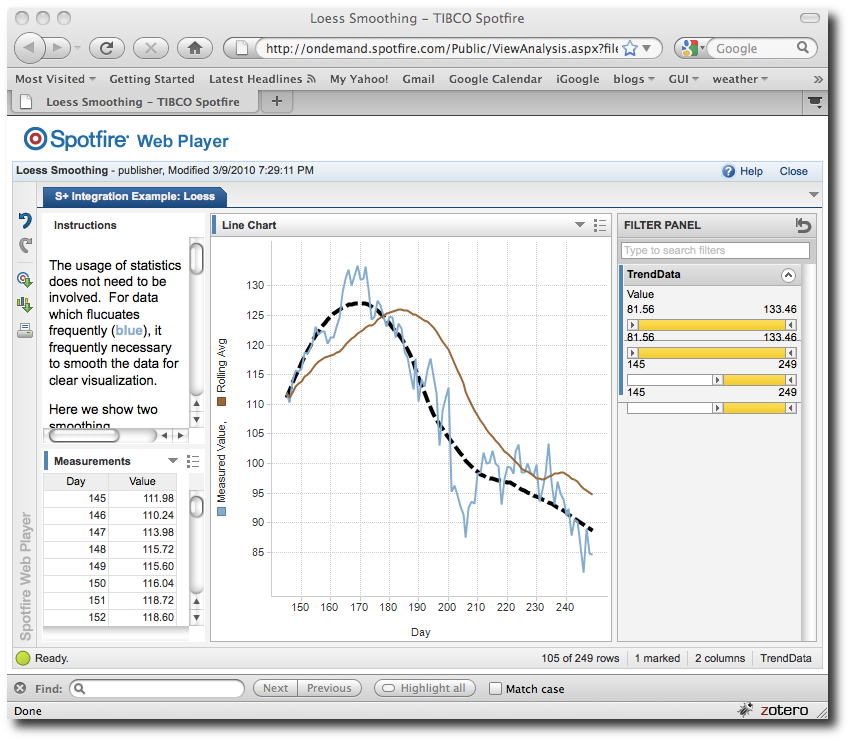
\includegraphics[width=0.8\textwidth]{fig-spotfire}
  \caption{A screen shot from Tibco's Spotfire web player illustrating
    a table widget (lower left), displaying the cases that are
    summarized in the graphic. The right bar filters the cases in the table. }
  \label{fig:GUI:spotfire}
\end{figure}


% \begin{figure}
%   \centering
% %%  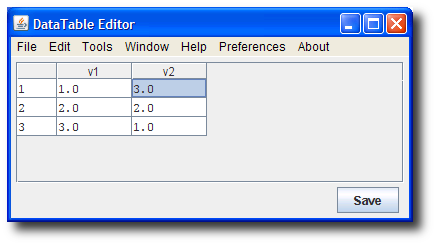
\includegraphics[width=.4\textwidth]{JGR-data-editor}
%   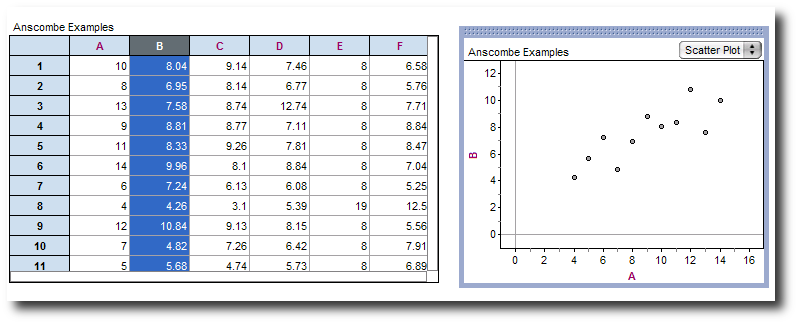
\includegraphics[width=.55\textwidth]{fathom-2-1-xyplot}
%   \caption{
%     Two windows showing the use of table widgets.
%     %%
    
% %     The left graphic shows the data editor from \pkg{JGR} using the
% %     table widget in Java.  
%     %%
%     The right graphic shows a data table and a graph in Fathom 2.1
%     with two views of the same data. One view uses a table widget, the
%     other a graph. Changes to one or the other views cause an update
%     to the underlying model. This model then will notify its various
%     displays to update. This arrangement allows for dynamic linking of
%     the table and the graph.}
%   \label{fig:GUI:table-widgets}
% \end{figure}

\subsubsection{Tree widgets}
\label{sec:GUI:tree-widgets}

So far, we have seen how list boxes display homogeneous vectors of
data, and how table widgets display tabular data, like that in a data
frame. Other widgets support the display of more complex data
structures. If the data has a hierarchical structure, then a \dfn{tree
  widget} may be appropriate for its display. Examples of hierarchical
data in \R\/ are directory structures, the components of a list, or
class hierarchies. The object browser in \pkg{JGR} uses a tree widget
to show the components of the objects in a user session
(Figure~\ref{fig:GUI:R-guis-exs-JGR}). The root node of the tree is
the ``data'' folder, and each data object in the global workspace is
treated as an offspring of this root node. For the data frame
\code{iraq}, its variables are considered as offspring of the data
frame. In this case these variables have no further offspring, as
indicated by the ``page'' icon.

%%%%%%%%%%%%%%%%%%%%%%%%%%%%%%%%%%%%%%%%%%%%%%%%%% 
\subsection{Displaying and editing text}
\label{sec:GUI:text-widgets}

The letter \acronym{P} in \acronym{WIMP} stands for ``pointer,'' so it
is unsurprising that \acronym{WIMP} GUIs are designed around the
pointing device. The keyboard is generally relegated to a secondary
role, in part because it is difficult to both type and move the mouse
at the same time. For statistical GUIs, especially when integrating
with the command-line interface of \R\/, the flexibility afforded by
arbitrary text entry is essential for any moderately complex
GUI. Toolkits generally provide separate widgets for text entry
depending on whether the editor supports a single line or multiple
lines.

\subsubsection{Single line text}
\label{sec:GUI:single-line-text}

A text entry widget for editing a single line of text is found in the
KDE print dialog (Figure~\ref{fig:GUI:print-dialogs}). It specifies
the page range. Specifying a complex page range, which might include
gaps, would require a complex point-and-click interface. In
order to avoid complicating the GUI for a feature that is rarely
useful, a simple language has been developed for specifying page
ranges. There is overhead involved in the parsing and validation of
such a language, but it is still preferable to the alternative.

\subsubsection{Text edit boxes}
\label{sec:GUI:textboxes}

Figure~\ref{fig:GUI:R-guis-exs-Rcmdr} shows three multi-line text
entries in an \pkg{Rcmdr} window. It provides an \R\/ console and
status message area. The ``Output Window'' demonstrates the utility of
formatting attributes. In this case, attributes specify the color of
the commands, so that the input can be distinguished from the output.



\begin{figure}
  \centering
  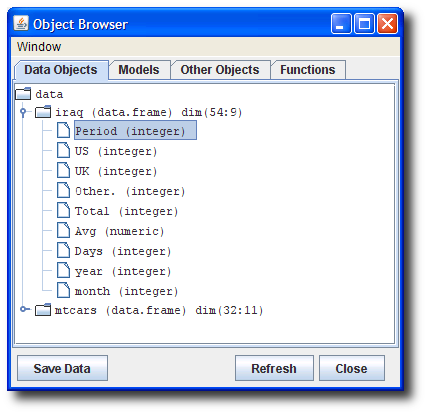
\includegraphics[width=.6\textwidth]{JGR-object-browser}
 \caption{
   The object browser in the \pkg{JGR} GUI
   using a tree widget 
   to display the possibly hierarchical nature of \R\/ objects.
   }
 \label{fig:GUI:R-guis-exs-JGR}
\end{figure}


\XXX{Not needed here?}
% %% A table showing the values and constructors
% %% Make changes to gnumeric spreadsheet, export
% {\small
% \newcommand{\PARASIZE}{1.25in}
% \newcommand{\LARGEPARASIZE}{1.45in}
% \begin{landscape}
%   \begin{table}[tbp]
%     \centering
%     \begin{minipage}{1.0\textwidth}
%       \begin{tabular}{lp{\PARASIZE}@{\quad}p{\LARGEPARASIZE}@{\quad}p{\PARASIZE}@{\quad}p{\PARASIZE}@{\quad}p{\PARASIZE}@{\quad}c}
%         %%
%         Widget & \code{gWidgets} & \code{RGtk2} & \code{RwxWidgets} &
%         \code{tcltk}\footnote{Some constructors require add-on
%           libraries, as indicated by parentheses.} & \code{rJava} &\\
%         \hline
%         \SweaveInput{widgets-constructors}
%       \end{tabular}
%     \end{minipage}
%     \caption{A table listing several common widgets with a constructor for
%       different toolkits discussed in the text.}
% \label{tab:GUI:widgets-constructors}
%   \end{table}
% \end{landscape}
% }

%%%%%%%%%%%%%%%%%%%%%%%%%%%%%%%%%%%%%%%%%%%%%%%%%% 
\subsection{Guides and feedback}
\label{sec:GUI:info-display}

Some widgets display information but do not respond to user
input. Their main
purpose is to guide and the user through the GUI and to display
feedback and status messages. Communicating application status, such
as during long-running calculations or when errors occur, is an often
over-looked but critically important feature of any effective GUI. 

\subsubsection{Labels}
\label{sec:GUI:labels}
%% Static Text
A label is a widget for placing text into a GUI that is typically not
intended for editing, or even selecting with a mouse. The main role of
a label is to describe another component of the GUI. Most toolkits
support rich text in labels. Figure~\ref{fig:GUI:R-guis-exs-Rcmdr}
shows labels marked in red and blue in \pkg{tcltk}.

\subsubsection{Statusbars}
\label{sec:GUI:statusbars}

A statusbar displays general status messages, as well as feedback on
actions initiated by the user, such as progress or errors. Messages
replace the previous message and may disappear after a certain period
of time. In the traditional document-oriented GUI, statusbars are
placed at the bottom.

Related to status bars are info bars or alert boxes, that allow a
programmer to display a transient message dialog that emerges from one
either the top or bottom the application window. An example is the
Firefox dialog that asks whether Firefox should remember a
password entered on the previous page. It appears just below the
toolbar and disappears automatically as the user continues to browse.

\subsubsection{Tooltips}
\label{sec:GUI:basic-tooltips}

A tooltip is a small window that is displayed when a user hovers their
mouse over a tooltip-enabled widget. These are an embellishment for
providing extra information about a particular piece of content
displayed by a widget. A common use-case is to guide new users of a
GUI. Many toolkits support the display of interactive hypertext in a
tooltip, which allows the user to request additional details.

\subsubsection{Progress bars}

A progress bar indicates progress on a particular task, which may or
may not be bounded. A bounded progress bar usually reports progress in
terms of percentage completed. Progress bars should be familiar, as
they are often displayed during software installation and while
downloading a file. For long-running statistical procedures they can
give useful feedback to the user that something is happening.

%% combined with modal dialogs
% \subsection{Choosers}
% \label{sec:GUI:choosers}

% Certain standard widgets are used to select values from a range
% defined by the system the user is on.


% \subsubsection{Color choosers}
% \label{sec:GUI:color-pickers}

% A color picker allows the selection of a color. 

% \subsubsection{Font choosers}
% \label{sec:GUI:font-choosers}

% A font chooser allows the selection of a font. 


\begin{figure}
  \centering
 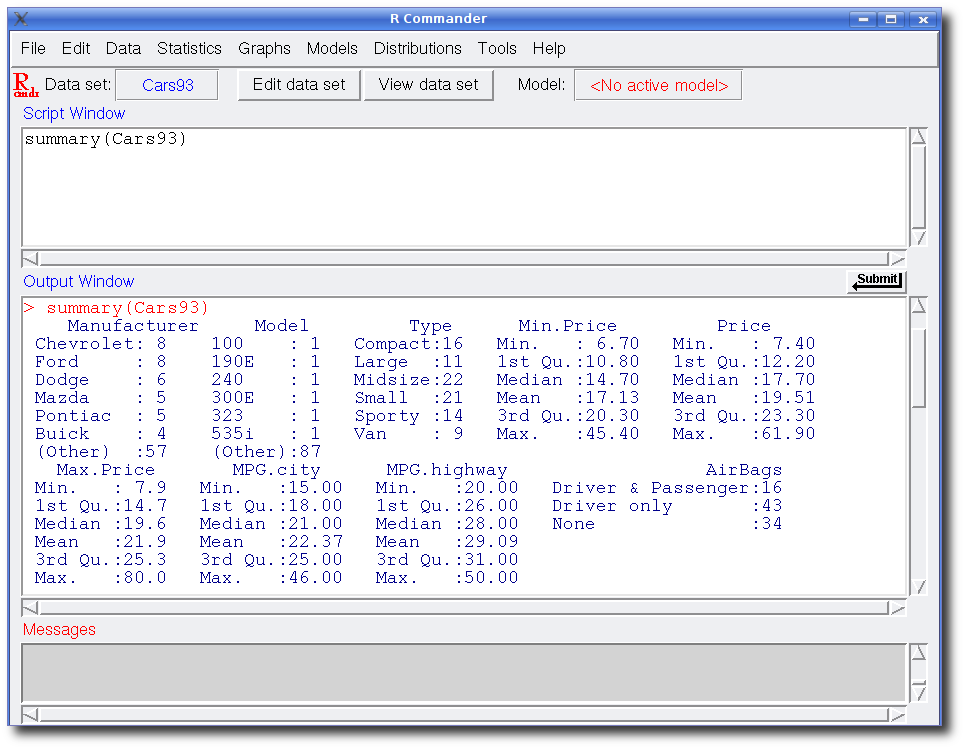
\includegraphics[width=.8\textwidth]{Rcmdr-main-window}
  \caption{
    Screenshot showing the main Rcmdr (1.3-11) window
    illustrating the use of multi-line text entry areas for a command
    area, an output area and a message area.}
  \label{fig:GUI:R-guis-exs-Rcmdr}
\end{figure}

\section{Containers}
\label{sec:GUI:basic-components-containers}
%% Containers

%%% FIXME: move to \paragraph{} instead of \subsubsection{}?

%% ML: Layout management is orthogonal to the type of container. This
%% is made obvious in the design of Swing and Qt: there is a separate
%% class hierarchy for layout managers, which are assigned to
%% container widgets. The container could be invisible or provide an
%% interface around its children, as with a frame, notebook or top-level
%% window. Thus, in Qt, a frame container could lay out its children
%% as a box, a grid, etc. I suggest discussing container types first,
%% and then discuss layout management policies, explaining that some
%% toolkits have widgets specific to a particular policy (and so
%% require a lot of nesting), while in others any container type is
%% capable of any type of layout.


%% JV: good point. 
% Widgets are arranged in a window to produce a GUI. Container widgets
% manage the layout. The simplest containers are like boxes
% that get packed in left to right or top to bottom. These boxes may be
% decorated with a frame or label, or may have some means of being
% hidden or displayed by the user. The nesting of box containers can
% provide a great deal of flexibility, but usually not
% enough. An example of a more flexible layout strategy is to position
% widgets on a grid.

%% Widget Hierarchy

The KDE print dialog of Figure~\ref{fig:GUI:print-dialogs} contains
many of the widgets we discussed in the previous section. Before we
can create such a dialog, we need to introduce how to position widgets
on the screen. This process is called \textit{widget layout}.

\ilayout{widget hierarchy}
A layout emerges from the organization of the widgets into a
hierarchy, where a parent widget positions its children within its
allocated space.  The top-level window is parentless and forms the
root of the hierarchy. A parent visually contains its children and
thus is usually called a \defn{container}. This design is natural,
because almost every GUI has a hierarchical layout. It is easy to
apply a different layout strategy to each region of a GUI, and when a
parent is added or removed from the GUI, so are its children.

It is sometimes tempting for novices to simply assign a fixed position
and dimensions for every widget in a GUI. However, such static layouts
do not scale well to changes in the state of the application or simply
changes to the window size dictated by the window manager. Thus, it is
strongly encouraged to delegate the responsibility of layout to a
\defn{layout manager} that dynamically calculates the layout as
constraints change. Depending on the toolkit, the layout manager might
be the container itself, or it might be a separate object to which the
container delegates.

Regardless, the type of layout is generally orthogonal to the type of
container. For example, a container might draw a border around its
children, and this would be independent of how its children are laid
out.  The rest of this section is divided into two parts: container
widgets and layout algorithms. We will continually refer back to the
KDE print dialog example as we proceed.

% The Apple guidelines\footcite[Ch. 15]{APPLE:HIG} suggest using ``center
% equalization'' for arranging widgets within a window. This means that
% the visual weight is balanced between the right and left side of the
% content area. This is not the case with the KDE print dialog.

\subsection{Containers}
\label{sec:containers}

\subsubsection{Top level windows}
\label{sec:GUI:top-level-windows}

The top-level window of a GUI is the root of the container
hierarchy. All other widgets are contained within it.  The
conventional main application window will consist of a menubar, a
tool bar and a status bar. The primary content of the window is
inserted between the tool bar and the status bar, in an area known as
the \dfnref{client area} or \dfnref{content area}. In the case of a
dialog, the content usually appears above a row of buttons, each of
which represent a possible response. The print dialog conforms to the
dialog convention. The print options fill the content area, and there
is a row of buttons at the bottom for issuing a response, such as
``Print''.

A window is typically decorated with a title and buttons to iconify,
maximize, or close. In the case of the print dialog, the top-level
window is entitled ``Print -- KPDF.''. Besides the text of the title,
the decorations are generally the domain of the window manager (often
part of the operating system). The application controls the contents
of the window.

Once a window is shown, its dimensions are managed by the user,
through the window manager. Thus, the programmer must size the window
before it becomes visible. This is often referred to as the
``default'' size of the window. Positioning of a top-level window is
generally left to the window manager.

The top-level window forwards window manager events to the
application. For example, an application might listen to the window
close event in order to prompt a user if there are any unsaved changes
to a document.

% Table~\ref{tab:GUI:containers-constructors} lists them
% together and provides the constructor name for the different toolkits
% discussed in this book.

\subsubsection{Tabbed notebooks}
\label{sec:GUI:notebooks}

A notebook widget depicts each child as if it were a page in a 
notebook. A
page is selected by clicking on a button that appears as a tab. Only a
single child is shown at once. The tabbed notebook is a space
efficient, categorizing container that is most appropriate when a user
is only interested in one page at a time. Modern web browsers take
advantage of it to allow several web pages to be open at once within
the same window. In the KDE print dialog, detailed options are
collapsed into a notebook in order to save space and organize the
multitude of options into simple categories: ``Copies'', ``Advanced
Options'', and ``Additional Tags''.

% %% A table showing the values and constructors
% %% Make changes to gnumeric spreadsheet, export
% {\small
% \newcommand{\PARASIZE}{1.25in}
% \begin{landscape}
%   \begin{table}
%     \centering
%     \caption{A table listing several containers with a constructor for the
%     different toolkits discussed in the text.}
%     \begin{tabular}{lp{\PARASIZE}@{\quad}p{\PARASIZE}@{\quad}p{\PARASIZE}@{\quad}p{\PARASIZE}@{\quad}p{\PARASIZE}@{\quad}c}
%       Widget & \code{gWidgets} & \code{RGtk2} & \code{RwxWidgets} &
%       \code{tcltk} & \code{rJava} &\\
%       \hline
%       \SweaveInput{containers-constructors}
%     \end{tabular}
%     \label{tab:GUI:containers-constructors}
%   \end{table}
% \end{landscape}
% }

\subsubsection{Frames}
\label{sec:GUI:frames}

A frame is a simple container that draws a border, possibly with a
label, around its child. The purpose of a frame is to enhance
comprehension of a GUI by visually distinguishing one group of
components from the others. The displayed page of the notebook in
Figure~\ref{fig:GUI:print-dialogs} contains two frames, visually
grouping widgets by their function: either \code{Page Selection}
or \code{Output Settings}.

\subsubsection{Expanding boxes}
\label{sec:GUI:expanding-boxes}

An expanding container, or box, will show or hide its children, according to the
state of a toggle button. By way of analogy, radio buttons are to
notebooks as check buttons are to expanding containers. An expanding box
allows the user to adapt a GUI to a particular use case or mode of
operation. Often, an expanding box contains so-called ``advanced''
widgets that are only occasionally useful and are only of interest to
a small subset of the users. For example, the \code{Options} button in
Figure~\ref{fig:GUI:print-dialogs} controls an expanding box that
contains the print options, which are usually best left to their
defaults.

\subsubsection{Paned boxes}
\label{sec:GUI:paned-boxes}

Usually, a layout manager allocates screen space to widgets, but
sometimes the user needs to adapt the allocation, according to a
present need. For example, the user may wish to increase the size of
an image to see the fine details. The \dfnref{paned container}
supports this by juxtaposing panes, either vertically (stacked) or
horizontally. The area separating the panes, sometimes called a
\dfnref{sash}, can be adjusted by the user with the mouse.
   
\subsection{Layout algorithms}
\label{sec:GUI:layout}

\subsubsection{Box layout}
\label{sec:GUI:Box-containers}

\ilayout{box layout}The box layout is the most common type of layout algorithm for
positioning child components. A box will pack its children either
horizontally or vertically\footnote{The \code{pack} command of
  \pkg{tcltk} can mix the two directions}. Usually, the widgets are
packed from left to right, for horizontal boxes, or from top to
bottom, in the case of a vertical box.  The upper left figure in
Figure~\ref{fig:GUI:box-possibilities} illustrates these possibilities.

\ilayout{resizing}The box layout needs to allocate space to its children in both the
vertical and horizontal directions. The typical box layout algorithm
begins by satisfying the minimum size requirements of its
children. The box may need to request more space for itself in order
to meet the requirements. 

Once the minimum requirements are satisfied, it is conventional and
usually desirable for the widgets to fill the space in the direction
orthogonal to the packing. For example, widgets in a horizontal box
will fill all of their vertical space (the upper right graphic in
Figure~\ref{fig:GUI:box-possibilities} shows some fill
possibilities). When this is not desired, most box widgets support
different ways of vertically (or horizontally) aligning the widgets
(the lower left graphic in Figure~\ref{fig:GUI:box-possibilities}).

More complex logic is involved in the allocation of space in the
direction of packing. Any available space after meeting minimum
requirements needs to be either allocated to the children or left
empty. This depends on whether any children are set to expand. The
available space will be distributed evenly to all expanding
children. Each child may fill that space or leave it empty. The
non-expanding children are simply packed against their
side of the container. If there are no expanding children, the
remaining space is left empty in the middle (or end if there are no
widgets packed against the other side). See the lower right
panel in Figure~\ref{fig:GUI:box-possibilities}. One could think
of this space being occupied by an invisible \ilayout{spring}spring. Invisible
expanding widgets also act as springs.


\begin{figure}
  \centering
  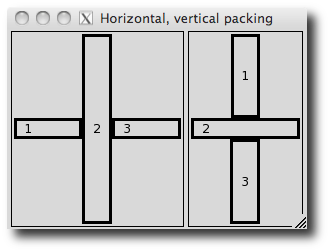
\includegraphics[width=.40\textwidth]{fig-basics-hor-ver}
  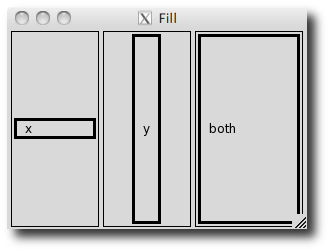
\includegraphics[width=.40\textwidth]{fig-basics-fill}\\
  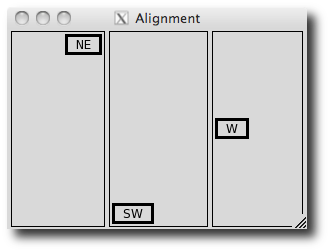
\includegraphics[width=.40\textwidth]{fig-basics-alignment}
  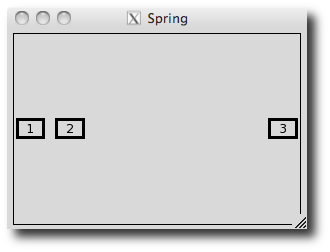
\includegraphics[width=.40\textwidth]{fig-basics-spring}
  \caption{
   %% 
    Different possibilities for packing child components within
    a box. 
    %% 
    The upper left shows horizontal and vertical layout.
    %% 
    The upper right shows some possible alignments or anchorings.
    %% 
    The lower left shows that a child could ``expand'' to fill the space
    either horizontally, vertically, or both.
    %% 
    The lower right shows both a fixed amount of space between the
    children and an expanding spring between the child components.  }
  \label{fig:GUI:box-possibilities}
\end{figure}

The button box in the KDE print dialog shows five buttons as child
components. At first glance the sizing appears to show that each
button is drawn to fully show its label with some fixed space placed
between the buttons. If the dialog is expanded, it is seen that there
is a spring between the 3rd and 4th buttons, so that the first 3 are
aligned with the left side of the window and the last two the right
side.

\subsubsection{Grid layout}
\label{sec:GUI:grid-layout}

The box layout algorithm only aligns its children along a single
dimension. The horizontal box, for example, vertically aligns its
children. Nevertheless, nesting permits the construction of complex
layouts using only simple boxes. However, it is sometimes desirable to
align widgets in both dimensions, i.e., to lay them out on a
\ilayout{grid layout}grid. The
most flexible grid layout algorithms allow non-regular sizing of rows
and columns, as well as the ability for a widget to span multiple
cells. Usually, a widget fills the cells allocated to it, but if this
is not possible, it may be anchored at a specific point within its
cell. 

The widgets in the ``Printer'' frame of
Figure~\ref{fig:GUI:box-possibilities} are subject to a grid layout
with five columns and six rows. The first row begins with the
``Name:'' label, and each widget in that row occupy a separate
column. This exposes the size of each column. The first column has
only labels, with text justified to the left.  The labels are aligned
horizontally to each other and vertically with the adjacent field.


% \section{End of chapter notes}
% \label{sec:GUI:end-of-chapter}
% \XXX{ fill this in }

% More documentation on GUIs is available in book format or online. 

% For \GTK\/ there is the gtk tutorial (pygtk); GTK API; DTL's notes; example
% code in the \pkg{RGtk2} package; php-gtk cookbook

% For \wxWidgets the book; DTL omegahat pages; wxWidgets API;

% For \tcltk\/ ActiveStates API; wettenhall examples (sciviews);
% Dalgaard's papers; R mailing list; book

% For \Java\/ Sun's website tutorials; API; rJava package page; 

% Event loops




%%%%%%%%%%%%%%%%%%%%%%%%%%%%%%%%%%%%%%%%%%%%%%%%%%

